\documentclass{article}%
\usepackage{preamble}
\usepackage[final]{pdfpages}

\begin{document}
\section{Introduction}
The Cerebrospinal Fluid (CSF) surrounds the brain and acts as a protection to the brain inside the skull. As a result of the cardiac cycle the CSF will flow up and down the subarachnoid space (SAS) surrounding the spinal cord. The Chiari malformation is a displacement of the cerebellar tonsils that partially blocks CSF flow entering the SAS around the spinal cord. This causes abnormal CSF flows which sometimes results in in a syringomyelia inside the spinal cord filled with fluid. Treatment may include surgery to remove parts of the bones of the skull to relieve pressure. Studies have shown that the syrinx gradually vanishes after surgery. The mechanisms behind this are not yet fully understood. Many researchers have suggested Computational Fluid Dynamics (CFD) to give useful insight, as experiments is very difficult and expensive. 
\\

\section{Problem definition}
The model consists of a spinal cord surrounded by space filled with CSF. \\ \\ 
\hspace*{2cm}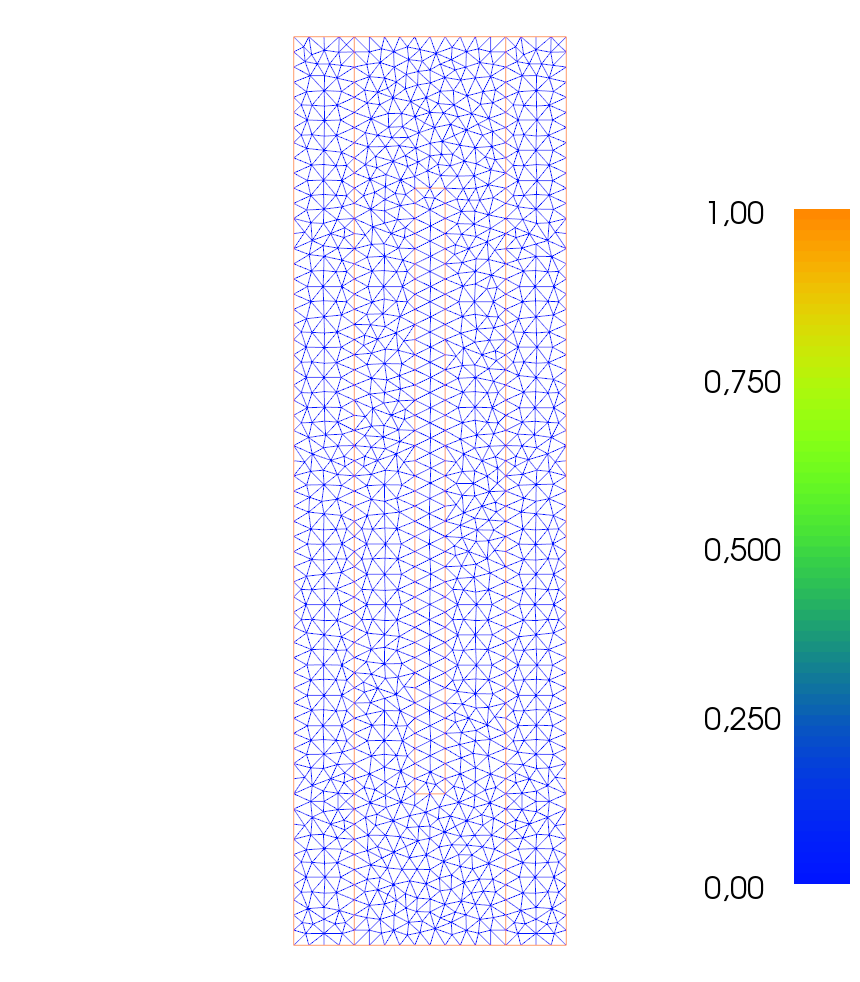
\includegraphics[scale=0.2]{mesh}
\\ \\
The cord has a diameter of 10 mm and the fluid space has a diameter of 18 mm. The model also has a inner central spinal canal, 2 mm in diameter. The central spinal canal has height 4 cm and is placed in the center of the mesh which has heigth 6 cm. \\

\end{document}
